\chapter{Background}
\label{ch:background}

\section{Associated graded objects}
\label{sctn:assoc-graded}

\begin{defn}
A filtered object $A$ consists of a finite chain
\[
A = F_0 A \supseteq F_1 A \supseteq F_2 A \supseteq \cdots
\supseteq F_{p-1} A \supseteq F_p A = 0
\]
of inclusions descending from $A$ to $0$.
\end{defn}

We will only consider finite chains because these are the examples
that arise in our Adams spectral sequences.  Thus we do not need
to refer to ``exhaustive" and ``Hausdorff" conditions on filtrations,
and we avoid subtle convergence issues associated with infinite filtrations.

\begin{ex}
\label{ex:14,8-filtered}
The $\C$-motivic stable homotopy group $\pi_{14,8} = \Z/2 \oplus \Z/2$
is a filtered object under the Adams filtration.  
The generators of this group are $\sigma^2$ and $\kappa$.
The subgroup $F_5$ is zero, the subgroup $F_3 = F_4$ is generated
by $\kappa$, and the subgroup $F_0 = F_1 = F_2$ is generated by
$\sigma^2$ and $\kappa$.
\end{ex}

\begin{defn}
Let $A$ be a filtered object.  The associated graded object
$\Gr A$ is
\[
\bigoplus_0^p F_i A / F_{i+1} A.
\]
\end{defn}

If $a$ is an element of $\Gr A$, then
we write $\{a\}$ for the set of elements of $A$ that are detected
by $a$.  In general, $\{a\}$ consists of more than one element of $A$,
unless $a$ happens to have maximal filtration.  
\revv{In other words}, the element $a$ is a coset $\alpha + F_{i+1} A$
for some $\alpha$ in $A$,
and $\{a\}$ is another name for this coset.
In this situation, we say that $a$ detects $\alpha$.

In this manuscript, the main example of a filtered object is
a $\C$-motivic homotopy group $\pi_{p,q}$, equipped with its Adams
filtration.  

\begin{ex}
\label{ex:14,8-assoc-graded}
Consider the $\C$-motivic stable homotopy group $\pi_{14,8}$
with its Adams filtration, as described in Example \ref{ex:14,8-filtered}.
The associated graded object is non-trivial only in degrees
$2$ and $4$, and it is generated by $h_3^2$ and $d_0$ respectively.
\end{ex}

\begin{defn}
Let $A$ and $B$ be filtered objects, perhaps with filtrations
of different lengths.
A map $f:A \map B$ is filtration preserving if
$f(F_i A)$ is contained in $F_i B$ for all $i$.
\end{defn}

Let $f: A \map B$ be a filtration preserving map of filtered objects.
We write $\Gr f: \Gr A \map \Gr B$ for the induced
map on associated graded objects.



\begin{defn}
\label{defn:hidden-value}
Let $a$ and $b$ be elements of $\Gr A$ and $\Gr B$ respectively.
We say that $b$ is the (not hidden) value of $a$ under $f$ if
$\Gr f(a) = b$.

We say that $b$ is the hidden value of $a$ under $f$ if:
\begin{enumerate}
\item
$\Gr f (a) = 0$.
\item
\revv{
there exists an element $\alpha$ of $\{a\}$ in $A$ such that:
\begin{enumerate}
\item
$f(\alpha)$ is contained in $\{b\}$ in $B$, and 
\item
there is no element $\gamma$ in filtration strictly higher than
$\alpha$ such that $f(\gamma)$ is contained in $\{b\}$.
\end{enumerate}
}
\end{enumerate}
\end{defn}

The motivation for condition (2b) may not be obvious.
The point is to avoid situations in which condition (2a) is satisfied
trivially.
Suppose that 
there is an element $\gamma$ 
such that $f(\gamma)$ is contained in $\{b\}$.
Let $a$ be any element of $\Gr A$ 
whose filtration is strictly less than the filtration of $\gamma$.
Now let $\alpha$ be any element of $\{ a\}$ such that $f(\alpha) = 0$.
(It may not be possible to choose such an $\alpha$ in general,
but sometimes it is possible.)
Then $\alpha + \gamma$ is another element
of $\{a\}$ such that $f(\alpha + \gamma)$ is contained in $\{b\}$.
Thus $f$ takes some element of $\{a\}$ into $\{b\}$, but only because
of the presence of $\gamma$.  
Condition (2b) is designed to exclude
this situation.

\begin{ex}
\label{ex:14,8-hidden-defn}
We illustrate the role of condition (2b) 
in Definition \ref{defn:hidden-value} with a specific example.
Consider the map $\eta: \pi_{14,8} \map \pi_{15,9}$.
The associated graded map $\Gr(\eta)$ takes $h_3^2$ to $0$ and 
takes $d_0$ to $h_1 d_0$.

The coset $\{h_3^2\}$ in $\pi_{14,8}$ consists of two elements
$\sigma^2$ and $\sigma^2 + \kappa$.  
One of these elements is non-zero after multiplying by $\eta$.
(In fact, $\eta \sigma^2$ equals zero, and 
$\eta (\sigma^2 + \kappa) = \eta \kappa$ is non-zero, but
that is not relevant here.)
Conditions (1) and (2a) of Definition \ref{defn:hidden-value}
are satisfied, but condition (2b) fails because of the presence
of $\kappa$ in higher filtration.
\end{ex}

Suppose that $b$ is the hidden value of $a$ under $f$.  
It is typically the case that $f(\alpha)$ is contained in $\{b\}$ for every
$\alpha$ in $A$.  However, an even more complicated situation can occur
in which this is not true.

Suppose that $b_0$ is the hidden value of $a_0$ under $f$, and suppose
that $b_1$ is the (hidden or not hidden) value of $a_1$ under $f$.
Moreover, suppose that the filtration of $a_0$ is strictly lower than
the filtration of $a_1$, and the filtration of $b_0$
is strictly greater than the filtration of $b_1$.
In this situation, we say that the value of $a_0$ under $f$ crosses
the value of $a_1$ under $f$.

The terminology arises from the usual graphical calculus, in which 
elements of higher filtration are drawn above elements of lower filtration,
and values of maps are indicated by line segments, as in 
Figure \ref{fig:crossing-values}.

\begin{figure}[h!]
\caption{Crossing values}
\label{fig:crossing-values}

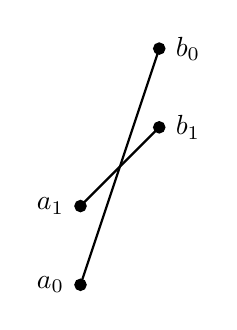
\begin{tikzpicture}[scale=0.5,
	every path/.style={line width=0.8pt},
	dot/.style={circle, inner sep=0, minimum size=0.13cm, draw=black,
				fill=black}]
	\node[dot, label=180:{$a_0$}] at (0,0) {};
	\draw (0,0) -- (2,6);
	\node[dot, label=180:{$a_1$}] at (0,2) {};
	\draw (0,2) -- (2,4);
	\node[dot, label=0:{$b_1$}] at (2,4) {};
	\node[dot, label=0:{$b_0$}] at (2,6) {};
	
\end{tikzpicture}

\end{figure}



\begin{ex}
For any map $X \map Y$ of $\C$-motivic spectra, naturality of the
Adams spectral sequence induces a filtration preserving map
$\pi_{p,q} X \map \pi_{p,q} Y$.
We are often interested in 
inclusion $S^{0,0} \map C\tau$ of the
bottom cell into $C\tau$, and in
projection $C\tau \map S^{1,-1}$ from $C\tau$ to the top cell.
We also consider the unit map
$S^{0,0} \map \mmf$.
\end{ex}

\subsection{Indeterminacy in hidden values}
\label{subsctn:hid-indet}

Definition \ref{defn:hidden-value} allows for the possibility of
some essentially redundant cases.  In order to avoid this redundancy,
we introduce indeterminacy into our definition.

Suppose, as in Definition \ref{defn:hidden-value},
that $b$ is the hidden value of $a$ under $f$, so
there exists some $\alpha$ in $\{a\}$ such that
$f(\alpha)$ is contained in $\{b\}$.
Suppose also that there is another element $a'$ in $\Gr A$ 
in degree strictly greater than the degree of $a$, such that
$f(\alpha')$ is contained in $\{b'\}$, where
$\alpha'$ is in $\{a'\}$ and $b'$ has the same degree as $b$.
Then $b+b'$ is also a hidden value of $a$ under $f$, since
$\alpha + \alpha'$ is contained in $\{a\}$ and
$f(\alpha + \alpha')$ is contained in $\{b+b'\}$.
In this case, we say that $b'$ belongs to the target
indeterminacy of the hidden value.

\begin{ex}
Consider the map $\eta: \pi_{63,33} \map \pi_{64,34}$.
The element $h_3 Q_2$ is a hidden value of $\tau h_1 H_1$
under this map.
This hidden value has target indeterminacy generated by 
$\tau h_1 X_2 = h_1 \cdot (\tau X_2 + \tau C')$.
\end{ex}


\subsection{Hidden extensions}

Let $\alpha$ be an element of $\pi_{a,b}$.  Then
multiplication by $\alpha$ induces a filtration preserving map
$\pi_{p,q} \map \pi_{p+a,q+b}$.
A hidden value of this map is precisely the same as a hidden
extension by $\alpha$ in the sense of \cite{Isaksen14c}*{Definition 4.2}.
For clarity, we repeat the definition here.

\begin{defn}
\label{defn:hidden}
Let $\alpha$ be an element of $\pi_{*,*}$ that is detected
by an element $a$ of the $E_\infty$-page of the $\C$-motivic Adams spectral sequence.
A hidden extension by $\alpha$ is a pair
of elements $b$ and $c$ of $E_\infty$ such that:
\begin{enumerate}
\item
$a b = 0$ in the $E_\infty$-page.
\item
There exists an element $\beta$ of $\{ b \}$ 
such that $\alpha \beta$ is contained in $\{ c \}$.
\item
If there exists an element $\beta'$ of $\{b'\}$ such
that $\alpha \beta'$ is contained in $\{ c\}$, then
the Adams filtration of $b'$ is less than or equal to the
Adams filtration of $b$.
\end{enumerate}
\end{defn}

A crossing value for the map 
$\alpha: \pi_{p,q} \map \pi_{p+a,q+b}$
is precisely the same
as a crossing extension in the sense of \cite{Isaksen14c}*{Examples
4.6 and 4.7}.

The discussion target indeterminacy
applies to the case of hidden extensions.
For example, the hidden $\eta$ extension from
$h_3 Q_2$ to $\tau h_1 H_1$ has target indeterminacy
generated by $\tau h_1 X_2$.

In later chapters, we will thoroughly explore hidden extensions
by $2$, $\eta$, and $\nu$.  We warn the reader that a complete
understanding of such hidden extensions does not necessarily
lead to a complete understanding of multiplication by
$2$, $\eta$, and $\nu$ in the $\C$-motivic stable homotopy groups.

For example, in the 45-stem, 
there exists an element $\theta_{4.5}$ that
is detected by $h_3^2 h_5$ such that $4 \theta_{4.5}$ is detected
by $h_0 h_5 d_0$.  This is an example of a hidden $4$ extension.
However, there is no hidden $2$ extension from
$h_0 h_3^2 h_5$ to $h_0 h_5 d_0$; condition (2b) of
Definition \ref{defn:hidden-value} is not satisfied.

In fact, a complete understanding of \emph{all} hidden
extensions leads to a complete understanding of the multiplicative
structure of the $\C$-motivic stable homotopy groups, but the process is
perhaps more complicated than expected.

For example, we mentioned in Example \ref{ex:14,8-hidden-defn}
that either $\eta (\sigma^2 + \kappa)$ or $\eta \sigma^2$ 
is non-zero, but these cases cannot be distinguished by a study
of hidden $\eta$ extensions.  However, we can express
that $\eta \sigma^2$ is zero by observing that there is
no hidden $\sigma$
extension from $h_1 h_3$ to $h_1 d_0$.

There are even further complications.  For example, 
the equation $h_2^3 + h_1^2 h_3 = 0$ does not prove that
$\nu^3 + \eta^2 \sigma$ equals zero because it could be detected
in higher filtration.  In fact, this does occur.  
Toda's relation \cite{Toda62} says that 
\[
\eta^2 \sigma + \nu^3 = \eta \epsilon,
\]
where $\eta \epsilon$ is detected by $h_1 c_0$.

We can express Toda's relation in terms of a ``matric hidden extension".
We have a map 
$[ \nu \quad \eta]: \pi_{6,4} \oplus \pi_{8,5} \map \pi_{9,6}$.
The associated graded map takes $(h_2^2, h_1 h_3)$ to zero,
but $h_1 c_0$ is the hidden value of $(h_2^2, h_1 h_3)$ under this 
map, in the sense of Definition \ref{defn:hidden-value}.

\section{Motivic modular forms}
\label{sctn:mmf}

Over $\C$, a ``motivic modular forms" spectrum $\mmf$
has recently been constructed \cite{GIKR18}.  
From our computational perspective, $\mmf$ is a ring spectrum
whose cohomology is $A//A(2)$, i.e., the quotient of the
$\C$-motivic Steenrod algebra by the subalgebra generated by
$\Sq^1$, $\Sq^2$, and $\Sq^4$.  By the usual change-of-rings
isomorphism, this implies that the homotopy groups of $\mmf$
are computed by an Adams spectral sequence whose $E_2$-page is
the cohomology of $\C$-motivic $A(2)$ \cite{Isaksen09}.  
The Adams spectral sequence for
$\mmf$ has been completely computed \cite{Isaksen18}.

By naturality, the unit map $S^{0,0} \map \mmf$ 
yields a map of Adams spectral sequences.  This map allows us
to transport information from the thoroughly understood
spectral sequence for $\mmf$ to the less well understood
spectral sequence for $S^{0,0}$.  This comparison technique
is essential at many points throughout our computations.

We rely on notation from \cite{Isaksen09} and \cite{Isaksen18}
for the Adams spectral sequence for $\mmf$, 
except that we use $a$ and $n$ instead of $\alpha$ and $\nu$
respectively.

For the most part, the map $\pi_{*,*} \map \pi_{*,*} \mmf$
is detected on Adams $E_\infty$-pages.  However, this map does
have some hidden values.

\begin{thm}
\label{thm:unit-mmf}
Through dimension 90, Table \ref{tab:unit-mmf} lists
all hidden values of the map $\pi_{*,*} \map \pi_{*,*} \mmf$.
\end{thm}

\begin{proof}
Most of these hidden values follow from hidden $\tau$ extensions
in the Adams spectral sequences for $S^{0,0}$ and for $\mmf$.
For example, for $S^{0,0}$, there is a hidden $\tau$ extension
from $h_1 h_3 g$ to $d_0^2$.  For $\mmf$, there is a hidden
$\tau$ extension from $c g$ to $d^2$.  This implies that
$c g$ is the hidden value of $h_1 h_3 g$.

A few cases are slightly more difficult.  
The hidden values of $\D h_1 h_3$ and $h_0 h_5 i$ follow from
the Adams-Novikov spectral sequences for $S^{0,0}$ and for $\mmf$.
These two values are detected on Adams-Novikov $E_\infty$-pages
in filtration $2$.

Next, the hidden value on $P h_2 h_5 j$ follows from 
multiplying the hidden value on $h_0 h_5 i$ by $d_0$.
Finally, the hidden values on $\D h_1^2 h_3$, $h_0 h_2 h_5 i$,
and $P h_5 j$ follow from already established hidden values,
relying on $h_1$ extensions and $h_2$ extensions.
\end{proof}

\begin{remark}
Through the 90-stem, there are no crossing values for the map
$\pi_{*,*} \map \pi_{*,*} \mmf$.  Moreover, in this range, there is only one hidden value that has target indeterminacy.
Namely, $\D^2 h_2 d$ is the hidden value of $P h_5 j$,
with target indeterminacy generated by $\tau^3 \D h_1 g^2$.
\end{remark}

\section{The cohomology of the $\C$-motivic Steenrod algebra}

We have implemented machine computations of
$\Ext$, i.e., 
the cohomology of the $\C$-motivic Steenrod algebra,
in detail through the 110-stem.  We take this computational data
for granted.  It is depicted graphically in the chart of the 
$E_2$-page shown in \cite{Isaksen14a}; the data is also available
there.
See \cite{Wang20} for a discussion of the implementation.

In addition to the additive structure of $\Ext$, we also have complete
information about multiplications by $h_0$, $h_1$, $h_2$, and $h_3$.
We do not have complete multiplicative information.  Occasionally we
must deduce some multiplicative information on an ad hoc basis.

Similarly, we do not have systematic machine-generated 
Massey product information about $\Ext$.  We deduce some of the 
necessary information about Massey products in Chapter \ref{ch:Massey}.

In the classical situation, Bruner has carried out extensive
machine computations of the cohomology of the classical Steenrod algebra
\cite{Bruner97}.  More recently, Bruner and Rognes have extended
these computations to total degree 184 \cite{BR20}.
This data includes complete primary multiplicative
information, but no higher Massey product structure.
We rely heavily on this information.
Our reliance on this data is so ubiquitous that we will not give
repeated citations.
\rev{Very recent work of Joey Beauvais-Feisthauer, Hood Chatham, Dexter Chua, and Weinan Lin
extends these machine computations of classical $\Ext$
to significantly higher stems.}

The May spectral sequence is the
key tool for a conceptual computation of $\Ext$.  
See \cite{Isaksen14c} for full details.  
In this manuscript, we use the May spectral sequence to
compute some Massey products that we need for various
specific purposes; see Remark \ref{rem:May-convergence}
for more details.

For convenience, we restate the following structural theorem
about a portion of $\Ext_\C$  \cite{Isaksen14c}*{Theorem 2.19}.

\begin{thm}
\label{thm:Chow-zero}
There is a highly structured isomorphism from 
$\Ext_\cl$ to the subalgebra of $\Ext$ consisting of elements in degrees 
$(s, f, w)$ with $s + f - 2w = 0$. 
This isomorphism takes classical elements of degree $(s,f)$ 
to motivic elements of degree $(2s+f,f,s+f)$.
\end{thm}

\section{Toda brackets}

Toda brackets are an essential computational tool for understanding
stable homotopy groups 
\revv{
\cite{Kochman90}*{Chapter 2}
\cite{Toda62} 
}.

Brackets appear throughout the various
stages of the computations, including in the analysis of Adams
differentials and in the resolution of hidden extensions.

It is well-known that the stable homotopy groups form a ring under
the composition product.  The higher Toda bracket structure is an
extension of this ring structure that is much deeper and more intricate.
Our philosophy is that the stable homotopy groups are not really
understood until the Toda bracket structure is revealed.

A complete analysis of all Toda brackets (even in a range)
is not a practical goal.  There are simply too many possibilities
to take into account methodically, especially when including
matric Toda brackets
(and possibly other more exotic non-linear types of brackets).
In practice, we compute only the Toda brackets that we need
for our specific computational purposes.


\subsection{The Moss Convergence Theorem}
\label{subsctn:Moss}

We next discuss the Moss Convergence Theorem \cite{Moss70}, which is
the essential tool for computing Toda brackets in stable homotopy
groups.  
\rev{See also \cite{BK21} for a modern proof of the Moss Convergence 
Theorem that applies not only in classical
stable homotopy theory but also to a wide variety of stable homotopy 
theories including $\C$-motivic stable homotopy theory.
}

In order to state the Moss Convergence Theorem precisely, 
we must clarify the
various types of bracket operations that arise.
First, the Adams $E_2$-page has Massey products 
arising from the fact that
it is the homology of the cobar complex, which is a 
differential graded algebra.  We typically refer to these
simply as ``Massey products", although we write
``Massey products in the $E_2$-page" for clarification when necessary.

Next, each higher $E_r$-page
also has Massey products, since it is the homology of the
$E_{r-1}$-page, which is a differential graded algebra.
We always refer to these as ``Massey products in the $E_r$-page"
to avoid confusion with the more familiar Massey products in
the $E_2$-page.  This type of bracket appears only occasionally 
throughout the manuscript.

Beware that the higher $E_r$-pages do not inherit Massey products
from the preceding pages.  For example, $\tau h_1^2$ equals the
Massey product $\langle h_0, h_1, h_0 \rangle$ in the $E_2$-page.
However, in the $E_3$-page, the bracket $\langle h_0, h_1, h_0 \rangle$
equals zero, since the product $h_0 h_1$ is already equal to zero
in the $E_2$-page before taking homology to obtain the $E_3$-page.

On the other hand, the Massey product $\langle h_1, h_0, h_3^2 \rangle$
is not a well-defined Massey product in the $E_2$-page since
$h_0 h_3^2$ is non-zero, while $\langle h_1, h_0, h_3^2 \rangle$
in the $E_3$-page equals $h_1 h_4$ because of the differential
$d_2(h_4) = h_0 h_3^2$.

Finally, we have Toda brackets in the stable homotopy groups
$\pi_{*,*}$.  The point of the Moss Convergence Theorem is to relate
these various kinds of brackets.


\revv{
\begin{defn}
\label{defn:crossing-diff}
Given $r$ and a degree $(s,f,w)$, 
a \textbf{crossing differential} is a nonzero differential
$d_{r+n}(x) = y$
in the $\C$-motivic Adams spectral sequence
 such that the stem of $y$ is $s$; the Adams filtration of $y$
is strictly greater than $f$ but strictly less than $f+n+1$;
and the weight of $y$ is $w$.
\end{defn}

\begin{remark}
In practice, we will never use Definition \ref{defn:crossing-diff}.
Rather, we will consider elements
$a$ and $b$ in the $E_{r}$-page of the $\C$-motivic Adams spectral sequence such that  $ab=0$.
We informally call a nonzero differential
$$d_{r+n}x=y$$
a crossing differential for the product 
$ab$ if it satisfies Definition \ref{defn:crossing-diff} for
the degree of $ab$.
In other words, 
the element $y$ has the same stem and motivic weight as the product $ab=0$; 
and the difference between the Adams filtration of $y$ and of
$ab$ is strictly greater than $0$ but strictly less than $n+1$.
\end{remark}
}


Figure \ref{fig:crossing-differentials} depicts the situation of 
a crossing differential in a chart for the $E_{r}$-page.
Typically, the product $ab$ is zero in the $E_{r}$-page because
it was hit by a $d_{r-1}$ differential, as shown by the dashed
arrow in the figure.  However, 
it may very well be the case that the product $ab$ is already zero in 
the $E_{r-1}$-page (or even in an earlier page),
in which case the dashed $d_{r-1}$ differential is actually 
$d_{r-1} (0) = 0$.

\begin{figure}[!ht]
\caption{Crossing differentials}
\label{fig:crossing-differentials}

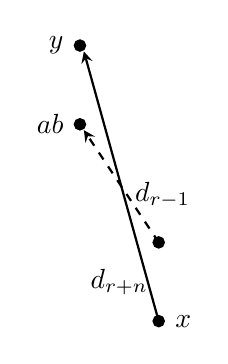
\begin{tikzpicture}[scale=0.5,
	>=stealth,
	every path/.style={line width=0.8pt},
	dot/.style={circle, inner sep=0, minimum size=0.13cm, draw=black,
				fill=black}]
	\node[dot, label=0:{$x$}] at (2,0) {};
	\draw[->] (2,0) -- (0.1,6.85);
	\node at (1,1) {$d_{r+n}$};
	\node[dot] at (2,2) {};
	\draw[->, dashed] (2,2) -- (0.1,4.85);
	\node at (2.1,3.2) {$d_{r-1}$};
	\node[dot, label=180:{$ab$}] at (0,5) {};
	\node[dot, label=180:{$y$}] at (0,7) {};
	
\end{tikzpicture}

\end{figure}


\begin{thm}[Moss Convergence Theorem]
\label{thm:Moss}
Suppose that $a$, $b$, and $c$ are permanent cycles in the $E_r$-page of the $\C$-motivic Adams spectral sequence that detect
homotopy classes $\alpha$, $\beta$, and $\gamma$ in $\pi_{*,*}$ respectively. Suppose further that
\begin{enumerate}
\item the Massey product $\langle a, b, c \rangle$ is defined in the 
$E_r$-page, i.e., $ab =0$ and $bc= 0$ in the $E_r$-page.
\item 
the Toda bracket $\langle \alpha, \beta, \gamma \rangle$ is defined in 
$\pi_{*,*}$, i.e., $\alpha \beta = 0$ and $\beta \gamma = 0$.
\item there are no crossing differentials for the products $ab$ and $bc$ in the $E_r$-page.
\end{enumerate}
Then there exists an element $e$ contained in the Massey product $\langle a, b, c \rangle$ in the $E_r$-page, such that
\begin{enumerate}
\item the element $e$ is a permanent cycle.
\item the element $e$ detects a homotopy class  in the Toda bracket	$\langle \alpha, \beta, \gamma \rangle$.	
\end{enumerate}
\end{thm}


\begin{remark}
The homotopy classes $\alpha$, $\beta$, and $\gamma$ 
are usually not unique.  The presence of elements in higher 
Adams filtration implies that $a$, $b$, and $c$ detect more
than one homotopy class.  Moreover, it may be the case that 
$\langle \alpha, \beta, \gamma \rangle$ is defined for only
some choices of $\alpha$, $\beta$, and $\gamma$, 
while the Toda bracket is not defined for other choices.
\end{remark}

\begin{remark}
The Moss Convergence Theorem \ref{thm:Moss} says that
a certain Massey product $\langle a, b, c \rangle$ in the $E_r$-page
contains an element with certain properties.
The theorem does not claim that every element of
$\langle a, b, c \rangle$ has these properties.  In the presence
of indeterminacies, there can be elements in $\langle a, b, c\rangle$
that do not satisfy the given properties.
\end{remark}

\begin{remark}
Beware that the Toda bracket $\langle \alpha, \beta, \gamma \rangle$
may have non-zero indeterminacy.  In this case,
we only know that $e$ detects one element of the Toda bracket.
Other elements of the Toda bracket could possibly be detected by
other elements of the Adams $E_\infty$-page; these occurrences must
be determined by inspection.
\end{remark}

\begin{remark}
In practice, one computes a Toda bracket
$\langle \alpha, \beta, \gamma \rangle$ by first studying
its corresponding Massey product $\langle a, b, c \rangle$ 
in a certain page of the Adams spectral sequence. 
In the case that the Massey product
$\langle a, b, c \rangle$ equals zero in the $E_r$-page
in Adams filtration $f$, 
the Moss Convergence Theorem \ref{thm:Moss}
does not imply that the Toda bracket 
$\langle \alpha, \beta, \gamma \rangle$ contains zero.  Rather,
the Toda bracket contains an element (possibly zero) that is detected
in Adams filtration at least $f+1$.
\end{remark}

\begin{ex}
Consider the Toda bracket $\langle \nu, \eta, \nu \rangle$.
The elements $h_1$ and $h_2$ are permanent cycles that detect 
$\eta$ and $\nu$, and the product $\eta \nu$ is zero.
We have that $\langle h_2, h_1, h_2 \rangle$ equals $h_1 h_3$,
with no indeterminacy, in the $E_2$-page.
There are no crossing differentials for the product $h_1 h_2 = 0$ 
in the $E_2$-page, so the Moss Convergence Theorem \ref{thm:Moss}
implies that  $h_1 h_3$ detects a homotopy class
in $\langle \nu, \eta, \nu \rangle$.

Note that $h_1h_3$ detects the homotopy class $\eta\sigma$ because
$h_3$ is a permanent cycle that detects $\sigma$. 
However, we cannot conclude that
$\eta\sigma$ is contained in $\langle \nu, \eta, \nu \rangle$. 
The presence of the permanent cycle $c_0$
in higher filtration means that $h_1 h_3$ detects both
$\eta \sigma$ and $\eta \sigma +\epsilon$, where $\epsilon$
is the unique homotopy class that is detected by $c_0$.
The Moss Convergence Theorem \ref{thm:Moss} implies that
either $\eta \sigma$ or $\eta \sigma + \epsilon$ is contained in
the Toda bracket $\langle \nu, \eta, \nu \rangle$.
In fact, $\eta \sigma + \epsilon$ is contained in the Toda bracket,
but determining this requires further analysis.
\end{ex}

\begin{ex}
Consider the Toda bracket $\langle \sigma^2, 2, \eta \rangle$.
The elements $h_3^2$, $h_0$, and $h_1$ are permanent cycles
that detect $\sigma^2$, $2$, and $\eta$ respectively, and
the products $2 \sigma^2$ and $2 \eta$ are both zero.
Due to the Adams differential $d_2(h_4) = h_0h_3^2$, the Massey product 
$\langle h_3^2, h_0, h_1 \rangle$ equals $h_1 h_4$ in the
$E_3$-page, with zero indeterminacy. 
There are no crossing differentials for the products $h_0 h_3^2 = 0$ 
and $h_0 h_1 = 0$ in the $E_3$-page.
The Moss Convergence Theorem \ref{thm:Moss} implies that
$h_1 h_4$ detects a homotopy class in the Toda bracket 
$\langle \sigma^2, 2, \eta \rangle$.

The element $h_3^2$ also detects $\sigma^2 + \kappa$, 
where $\kappa$ is the unique homotopy class that is detected by $d_0$,
and the product $2 (\sigma^2 + \kappa)$ is zero.
The Moss Convergence Theorem \ref{thm:Moss} also implies that
$h_1 h_4$ detects a homotopy class in the Toda bracket 
$\langle \sigma^2 + \kappa, 2, \eta \rangle$. 
\end{ex}

\begin{ex}
Consider the Toda bracket $\langle \kappa, 2, \eta \rangle$.
The elements $d_0$, $h_0$, and $h_1$ are permanent cycles
that detect $\kappa$, $2$, and $\eta$ respectively, and
the products $2 \kappa$ and $2 \eta$ are both zero.
Due to the Adams differential $d_3(h_0h_4) = h_0d_0$, 
the Massey product $\langle d_0, h_0, h_1 \rangle$ equals
$h_0 h_4 \cdot h_1 = 0$ in Adams filtration 3 in the $E_4$-page,
with zero indeterminacy.
There are no crossing differentials for the products $h_0 d_0 = 0$ 
and $h_0 h_1 = 0$ in the $E_4$-page.
The Moss Convergence Theorem \ref{thm:Moss} implies that
the Toda bracket $\langle \kappa, 2, \eta \rangle$ either contains zero,
or it contains a non-zero element detected in Adams filtration
greater than $3$.

The only possible detecting element is $P c_0$. 
There is a hidden $\eta$ extension from $h_0^3h_4$ to $P c_0$, 
so $P c_0$ detects an element in the indeterminacy of 
$\langle \kappa, 2, \eta \rangle$.
Consequently, the Toda bracket is $\{0, \eta \rho_{15} \}$,
where $\rho_{15}$ is detected by $h_0^3h_4$.
\end{ex}

\begin{ex}
The Massey product $\langle h_2, h_3^2, h_0^2 \rangle$
equals $\{f_0, f_0 + h_0^2 h_2 h_4 \}$ in the $E_2$-page.
The elements $h_2$, $h_3^2$, and $h_0^2$ are permanent cycles
that detect $\nu$, $\sigma^2$, and $4$ respectively, and
the products $\nu \sigma^2$ and $4 \sigma^2$ are both zero.
However, the product $h_0^2 h_3^2$ has a crossing differential
$d_3(h_0 h_4) = h_0 d_0$.
The Moss Convergence Theorem \ref{thm:Moss} does not apply,
and we cannot conclude anything about the Toda bracket
$\langle \nu, \sigma^2, 4 \rangle$.  In particular,
we cannot conclude that $\{f_0, f_0 + h_0^2 h_2 h_4\}$ 
contains a permanent cycle.  In fact, both elements support
Adams $d_2$ differentials.
\end{ex}

\begin{remark}
\label{rem:Moss-4fold}
There is a version of the Moss Convergence Theorem \ref{thm:Moss}
for computing fourfold Toda brackets 
$\langle \alpha, \beta, \gamma, \delta\rangle$ in terms of fourfold
Massey products $\langle a, b, c, d \rangle$ in the $E_r$-page. 
In this case, the crossing differential condition applies not only to
the products $ab$, $bc$, and $cd$, but also to the subbrackets
$\langle a, b, c \rangle$ and $\langle b, c, d \rangle$.
\end{remark}

\begin{remark}
\label{rem:May-convergence}
Just as the Moss Convergence Theorem \ref{thm:Moss} is the key
tool for computing Toda brackets with the Adams spectral sequence,
the May Convergence Theorem is the key tool for computing
Massey products with the May spectral sequence.  The statement of
the May Convergence Theorem is entirely analogous to the
statement of the Moss Convergence Theorem, with 
Adams differentials replaced by  May differentials;
 Adams $E_r$-pages replaced by 
May $E_r$-pages;  $\pi_{*,*}$ replaced by
 $\Ext$; and  Toda brackets replaced
by Massey products.  An analogous crossing differential
condition applies.  See \cite{Isaksen14c}*{Section 2.2} \cite{May69}
for more details.  We will use the May Convergence Theorem to
compute various Massey products that we need for specific purposes.
\end{remark}


\subsection{Moss's higher Leibniz rule}
\label{subsctn:Leibniz}

Occasionally, we will use Moss's higher Leibniz rule \cite{Moss70}, 
which describes how Massey products in the $E_r$-page interact with
the Adams $d_r$ differential.  This theorem is a 
direct generalization of the usual Leibniz rule
$d_r(ab) = d_r(a) b + a d_r(b)$ for twofold products.

\begin{thm}
\label{thm:Leibniz}
\cite{Moss70}
Suppose that $a$, $b$, and $c$ are elements in the $E_r$-page 
of the $\C$-motivic Adams spectral sequence such that $ab=0$, $bc=0$,
$d_r(b) a = 0$, and $d_r(b) c = 0$.
Then
$$d_r \langle a, b, c \rangle \subseteq \langle d_r(a), b, c \rangle + \langle a, d_r(b), c \rangle + \langle a, b, d_r(c) \rangle,$$	
where all brackets are computed in the $E_r$-page.
\end{thm}

\begin{remark}
By the Leibniz rule, 
the conditions $d_r (b) a = 0$ and $d_r (b) c =0$ imply that 
$d_r (a) b = 0$ and $d_r (c) b =0$. Therefore, all of the Massey
products in Theorem \ref{thm:Leibniz} are well-defined.
\end{remark}

\begin{remark}
The Massey products in Moss's higher Leibniz rule \ref{thm:Leibniz} may have indeterminacies,
so the statement involves an inclusion of sets, rather than an equality.
\end{remark}

\begin{remark}
Beware that Moss's higher Leibniz rule \ref{thm:Leibniz}
cannot be applied
to Massey products in the $E_r$-page to study differentials in
higher pages.  For example, we cannot use it 
to compute the $d_3$ differential on a Massey product in the $E_2$-page.
In fact, there are versions of the higher Leibniz rule that
apply to higher differentials \cite{Kochman78}*{Theorem 8.2} 
\cite{May69}*{Theorem 4.3}, 
but these results have strong
vanishing conditions that often do not hold in practice.
\end{remark}

\begin{ex}
\label{ex:Leibniz-tD1h1^2}
Consider the element $\tau \Delta_1 h_1^2$, which 
was called $G$ in \cite{Tangora70a}.
Table \ref{tab:Adams-d2} shows that there is an Adams
differential $d_2(\tau \Delta_1 h_1^2) = M h_1 h_3$, which follows
by comparison to $C\tau$.  To illustrate Moss's higher Leibniz
rule \ref{thm:Leibniz}, we shall give an independent derivation
of this differential.

Table \ref{tab:Massey} shows that $\tau \Delta_1 h_1^2$ equals
the Massey product $\langle h_1, h_0, D_1 \rangle$,
with no indeterminacy.
By Moss's higher Leibiz rule \ref{thm:Leibniz}, the element
$d_2(\tau \Delta_1 h_1^2)$ is contained in
\[
\langle 0, h_0, D_1 \rangle + \langle h_1, 0, D_1 \rangle + \langle h_1, h_0, d_2(D_1) \rangle.
\]
By inspection, the first two terms vanish.  Also, Table \ref{tab:Adams-d2}
shows that $d_2(D_1)$ equals $h_0^2 h_3 g_2$.

Therefore,
$d_2(\tau \Delta_1 h_1^2)$ is contained in the bracket
$\langle h_1, h_0, h_0^2 h_3 g_2 \rangle$, which equals
$\langle h_1, h_0, h_0^2 g_2 \rangle h_3$.
Finally, Table \ref{tab:Massey} shows that
$\langle h_1, h_0, h_0^2 g_2 \rangle$ equals $M h_1$.
This shows that 
$d_2(\tau \D_1 h_1^2)$ equals $M h_1 h_3$.	
\end{ex}



\begin{ex}
Consider the element  $\tau e_0 g$ in the Adams $E_3$-page.
Because of the Adams differential $d_2(e_0) = h_1^2 d_0$, we have that
$\tau e_0 g$ equals $\langle d_0, h_1^2, \tau g \rangle$ 
in the Adams $E_3$-page.
The higher Leibniz rule \ref{thm:Leibniz} implies that 
$d_3(\tau e_0 g)$ is contained in
\[
\langle 0, h_1^2, \tau g \rangle + \langle d_0, 0, \tau g \rangle +
\langle d_0, h_2^2, 0 \rangle,
\]
which equals $\{0, c_0 d_0^2 \}$.
In this case, 
the higher Leibniz rule \ref{thm:Leibniz} does not help to determine
the value of $d_3(\tau e_0 g)$ because the indeterminacy is too large.
(In fact, $d_3(\tau e_0 g)$ does equal $c_0 d_0^2$, but we need a 
different argument.)
\end{ex}

\begin{ex}
Lemma \ref{lem:d3-Dh2^2h6} shows that 
$d_3(\D h_2^2 h_6)$ equals $h_1 h_6 d_0^2$. 
This argument uses that 
$\D h_2^2 h_6$ equals $\langle \D h_2^2, h_5^2, h_0 \rangle$
in the $E_3$-page, because of the Adams differential 
$d_2(h_6) = h_0 h_5^2$.
\end{ex}

\subsection{Shuffling formulas for Toda brackets}

Toda brackets satisfy various types of formal relations that we 
will use extensively.  The most important example of such a relation
is the shuffle formula
\[
\alpha \langle \beta, \gamma, \delta \rangle =
\langle \alpha, \beta, \gamma \rangle \delta,
\]
which holds whenever both Toda brackets are defined.
Note the equality of sets here; the indeterminacies of both
expressions are the same.

The following theorem states some formal properties of threefold
Toda brackets that we will use later.  
We apply these results so frequently that
we typically use them without further mention.

\begin{thm}
\label{thm:Toda-3fold}
\revv{\cite{Toda62}*{p.\ 33}}
Let $\alpha$, $\alpha'$, $\beta$, $\gamma$, and $\delta$ 
be homotopy classes in $\pi_{*,*}$. 
Each of the following relations involving threefold Toda brackets
holds up to \rev{signs}, whenever the Toda brackets are defined:
\begin{enumerate}
\item 
$ \langle \alpha + \alpha', \beta, \gamma\rangle \subseteq 
\langle \alpha, \beta, \gamma \rangle + 
\langle \alpha', \beta, \gamma\rangle.$
\item 
$ \langle \alpha, \beta, \gamma\rangle = 
\langle \gamma, \beta, \alpha \rangle.$
\item
 $\alpha \langle \beta, \gamma, \delta \rangle \subseteq 
 \langle \alpha\beta, \gamma, \delta \rangle.$
\item 
$\langle \alpha  \beta, \gamma, \delta \rangle \subseteq 
\langle \alpha, \beta\gamma, \delta \rangle.$
\item $\alpha \langle \beta, \gamma, \delta \rangle = \langle \alpha, \beta, \gamma \rangle \delta.$
\item $0 \in \langle \alpha, \beta, \gamma\rangle + 
\langle \beta, \gamma, \alpha\rangle + 
\langle \gamma, \alpha, \beta\rangle.$
\item 
\label{part:0}
\rev{$0 \in \langle \langle \alpha, \beta, \gamma \rangle, \delta, \epsilon \rangle + \langle \alpha, \langle \beta, \gamma, \delta \rangle, \epsilon \rangle + \langle  \alpha, \beta, \langle \gamma, \delta, \epsilon \rangle \rangle.$}
\end{enumerate}
\end{thm}

\rev{
Part (\ref{part:0}) of
Theorem \ref{thm:Toda-3fold}
requires some further explanation.
In the expression
$\langle \langle \alpha, \beta, \gamma \rangle, \delta, \epsilon \rangle$,
we have a set $\langle \alpha, \beta, \gamma \rangle$ as the 
first input to a threefold Toda bracket.
The expression $\langle \langle \alpha, \beta, \gamma \rangle, \delta, \epsilon \rangle$ is defined to be the union of all sets of the form
$\langle \zeta, \delta, \epsilon \rangle$, where
$\zeta$ ranges over all elements of 
$\langle \alpha, \beta, \gamma \rangle$.
Similar remarks apply to the other terms in Part (\ref{part:0}).
} 



We next turn our attention to fourfold Toda brackets.  New complications
arise in this context.  If $\alpha \beta = 0$, $\beta \gamma = 0$,
$\gamma \delta = 0$, $\langle \alpha, \beta, \gamma \rangle$
contains zero, and $\langle \beta, \gamma, \delta \rangle$
contains zero, then the fourfold bracket
$\langle \alpha, \beta, \gamma, \delta \rangle$
is not necessarily defined.  Problems can arise when both
threefold subbrackets have indeterminacy.
See \cite{Isaksen14b} for a careful analysis of this problem in the
analogous context of Massey products.

However, when at least one of the threefold subbrackets is strictly
zero, then these difficulties vanish.  Every fourfold bracket that
we use has at least one threefold subbracket that is strictly zero.

Another complication with fourfold Toda brackets lies in the
description of the indeterminacy.  If at least one
threefold subbracket is strictly zero, then the indeterminacy of
$\langle \alpha, \beta, \gamma, \delta \rangle$
is the linear span of the sets
$\langle \alpha, \beta, \epsilon \rangle$,
$\langle \alpha, \epsilon, \delta \rangle$,
and $\langle \epsilon, \gamma, \delta \rangle$,
where $\epsilon$ ranges over all possible values in the appropriate
degree for which the Toda bracket is defined.

The following theorem states some formal properties of fourfold
Toda brackets that we will use later.  
We apply these results so frequently that
we typically use them without further mention.

\begin{thm}
\label{thm:Toda-4fold}
\revv{\cite{Kochman90}*{Chapter 2}}
Let $\alpha$, $\alpha'$, $\beta$, $\gamma$, $\delta$, and 
$\epsilon$ be homotopy classes in $\pi_{*,*}$. 
Each of the following relations involving fourfold Toda brackets
holds up to \rev{signs}, whenever the Toda brackets are defined:
\begin{enumerate}
\item $ \langle \alpha + \alpha', \beta, \gamma, \delta\rangle \subseteq  \langle \alpha, \beta, \gamma, \delta\rangle + \langle \alpha', \beta, \gamma, \delta\rangle.$
\item $ \langle \alpha, \beta, \gamma, \delta\rangle = \langle \delta, \gamma, \beta, \alpha \rangle.$
\item $\alpha \langle \beta, \gamma, \delta, \epsilon \rangle \subseteq \langle \alpha\beta, \gamma, \delta, \epsilon \rangle.$
\item $\langle \alpha  \beta, \gamma, \delta, \epsilon \rangle \subseteq \langle \alpha, \beta\gamma, \delta, \epsilon \rangle.$
\item $\alpha \langle \beta, \gamma, \delta, \epsilon \rangle = \langle \alpha, \beta, \gamma, \delta \rangle \epsilon.$
\item 
\label{part:a<b,c,d,e>}
$\alpha \langle \beta, \gamma, \delta, \epsilon \rangle \subseteq \langle \langle \alpha, \beta, \gamma \rangle, \delta, \epsilon \rangle.$
\end{enumerate}
\end{thm}

\rev{
As in Part (\ref{part:0}) of Theorem \ref{thm:Toda-3fold},
Part (\ref{part:a<b,c,d,e>}) of
Theorem \ref{thm:Toda-4fold}
requires some further explanation.
The expression $\langle \langle \alpha, \beta, \gamma \rangle, \delta, \epsilon \rangle$ is defined to be the union of all sets of the form
$\langle \zeta, \delta, \epsilon \rangle$, where
$\zeta$ ranges over all elements of 
$\langle \alpha, \beta, \gamma \rangle$.
}

We will make occasional use of matric Toda brackets. 
We will not describe their shuffling properties in detail, except to observe that
they obey analogous matric versions of the properties
in Theorems \ref{thm:Toda-3fold} and \ref{thm:Toda-4fold}. 
\revv{These properties can be proved with the same techniques that apply
to matric Massey product \cite{May69}; see 
\cite{Kochman78} \cite{Kochman96} for examples of this style of argument.} 







